\documentclass[twoside]{book}

% Packages required by doxygen
\usepackage{fixltx2e}
\usepackage{calc}
\usepackage{doxygen}
\usepackage[export]{adjustbox} % also loads graphicx
\usepackage{graphicx}
\usepackage[utf8]{inputenc}
\usepackage{makeidx}
\usepackage{multicol}
\usepackage{multirow}
\PassOptionsToPackage{warn}{textcomp}
\usepackage{textcomp}
\usepackage[nointegrals]{wasysym}
\usepackage[table]{xcolor}

% Font selection
\usepackage[T1]{fontenc}
\usepackage[scaled=.90]{helvet}
\usepackage{courier}
\usepackage{amssymb}
\usepackage{sectsty}
\renewcommand{\familydefault}{\sfdefault}
\allsectionsfont{%
  \fontseries{bc}\selectfont%
  \color{darkgray}%
}
\renewcommand{\DoxyLabelFont}{%
  \fontseries{bc}\selectfont%
  \color{darkgray}%
}
\newcommand{\+}{\discretionary{\mbox{\scriptsize$\hookleftarrow$}}{}{}}

% Page & text layout
\usepackage{geometry}
\geometry{%
  a4paper,%
  top=2.5cm,%
  bottom=2.5cm,%
  left=2.5cm,%
  right=2.5cm%
}
\tolerance=750
\hfuzz=15pt
\hbadness=750
\setlength{\emergencystretch}{15pt}
\setlength{\parindent}{0cm}
\setlength{\parskip}{3ex plus 2ex minus 2ex}
\makeatletter
\renewcommand{\paragraph}{%
  \@startsection{paragraph}{4}{0ex}{-1.0ex}{1.0ex}{%
    \normalfont\normalsize\bfseries\SS@parafont%
  }%
}
\renewcommand{\subparagraph}{%
  \@startsection{subparagraph}{5}{0ex}{-1.0ex}{1.0ex}{%
    \normalfont\normalsize\bfseries\SS@subparafont%
  }%
}
\makeatother

% Headers & footers
\usepackage{fancyhdr}
\pagestyle{fancyplain}
\fancyhead[LE]{\fancyplain{}{\bfseries\thepage}}
\fancyhead[CE]{\fancyplain{}{}}
\fancyhead[RE]{\fancyplain{}{\bfseries\leftmark}}
\fancyhead[LO]{\fancyplain{}{\bfseries\rightmark}}
\fancyhead[CO]{\fancyplain{}{}}
\fancyhead[RO]{\fancyplain{}{\bfseries\thepage}}
\fancyfoot[LE]{\fancyplain{}{}}
\fancyfoot[CE]{\fancyplain{}{}}
\fancyfoot[RE]{\fancyplain{}{\bfseries\scriptsize Generated by Doxygen }}
\fancyfoot[LO]{\fancyplain{}{\bfseries\scriptsize Generated by Doxygen }}
\fancyfoot[CO]{\fancyplain{}{}}
\fancyfoot[RO]{\fancyplain{}{}}
\renewcommand{\footrulewidth}{0.4pt}
\renewcommand{\chaptermark}[1]{%
  \markboth{#1}{}%
}
\renewcommand{\sectionmark}[1]{%
  \markright{\thesection\ #1}%
}

% Indices & bibliography
\usepackage{natbib}
\usepackage[titles]{tocloft}
\setcounter{tocdepth}{3}
\setcounter{secnumdepth}{5}
\makeindex

% Hyperlinks (required, but should be loaded last)
\usepackage{ifpdf}
\ifpdf
  \usepackage[pdftex,pagebackref=true]{hyperref}
\else
  \usepackage[ps2pdf,pagebackref=true]{hyperref}
\fi
\hypersetup{%
  colorlinks=true,%
  linkcolor=blue,%
  citecolor=blue,%
  unicode%
}

% Custom commands
\newcommand{\clearemptydoublepage}{%
  \newpage{\pagestyle{empty}\cleardoublepage}%
}

\usepackage{caption}
\captionsetup{labelsep=space,justification=centering,font={bf},singlelinecheck=off,skip=4pt,position=top}

%===== C O N T E N T S =====

\begin{document}

% Titlepage & ToC
\hypersetup{pageanchor=false,
             bookmarksnumbered=true,
             pdfencoding=unicode
            }
\pagenumbering{alph}
\begin{titlepage}
\vspace*{7cm}
\begin{center}%
{\Large My Project \\[1ex]\large 1 }\\
\vspace*{1cm}
{\large Generated by Doxygen 1.8.13}\\
\end{center}
\end{titlepage}
\clearemptydoublepage
\pagenumbering{roman}
\tableofcontents
\clearemptydoublepage
\pagenumbering{arabic}
\hypersetup{pageanchor=true}

%--- Begin generated contents ---
\chapter{Class Index}
\section{Class List}
Here are the classes, structs, unions and interfaces with brief descriptions\+:\begin{DoxyCompactList}
\item\contentsline{section}{\hyperlink{struct_node}{Node} }{\pageref{struct_node}}{}
\end{DoxyCompactList}

\chapter{File Index}
\section{File List}
Here is a list of all files with brief descriptions\+:\begin{DoxyCompactList}
\item\contentsline{section}{Code/\hyperlink{tut6__q3_8cpp}{tut6\+\_\+q3.\+cpp} \\*This program implements Bentley-\/\+Ottmann Algorithm to find all intersection of n given lines and also find linear fit }{\pageref{tut6__q3_8cpp}}{}
\end{DoxyCompactList}

\chapter{Class Documentation}
\hypertarget{struct_disjoint_sets}{}\section{Disjoint\+Sets Struct Reference}
\label{struct_disjoint_sets}\index{Disjoint\+Sets@{Disjoint\+Sets}}
\subsection*{Public Member Functions}
\begin{DoxyCompactItemize}
\item 
\hyperlink{struct_disjoint_sets_a26da401bf4e56a876533c97643c7d9c2}{Disjoint\+Sets} (int \hyperlink{struct_disjoint_sets_aeb43c9e003e2bd5b83b5c60d56dfd23e}{n})
\item 
int \hyperlink{struct_disjoint_sets_a14ff5306079945dd59c0c6d55129ac2e}{find} (int u)
\item 
void \hyperlink{struct_disjoint_sets_a349af3d249271920c355d9ef2a641f87}{merge} (int x, int y)
\end{DoxyCompactItemize}
\subsection*{Public Attributes}
\begin{DoxyCompactItemize}
\item 
int $\ast$ \hyperlink{struct_disjoint_sets_ad7f9caf9365a04a1c6670aa372a3cdbd}{parent}
\item 
int $\ast$ \hyperlink{struct_disjoint_sets_a93f26d80d2fb349bd97793fb41e502e8}{rnk}
\item 
int \hyperlink{struct_disjoint_sets_aeb43c9e003e2bd5b83b5c60d56dfd23e}{n}
\end{DoxyCompactItemize}


\subsection{Detailed Description}


Definition at line 38 of file q22.\+cpp.



\subsection{Constructor \& Destructor Documentation}
\mbox{\Hypertarget{struct_disjoint_sets_a26da401bf4e56a876533c97643c7d9c2}\label{struct_disjoint_sets_a26da401bf4e56a876533c97643c7d9c2}} 
\index{Disjoint\+Sets@{Disjoint\+Sets}!Disjoint\+Sets@{Disjoint\+Sets}}
\index{Disjoint\+Sets@{Disjoint\+Sets}!Disjoint\+Sets@{Disjoint\+Sets}}
\subsubsection{\texorpdfstring{Disjoint\+Sets()}{DisjointSets()}}
{\footnotesize\ttfamily Disjoint\+Sets\+::\+Disjoint\+Sets (\begin{DoxyParamCaption}\item[{int}]{n }\end{DoxyParamCaption})\hspace{0.3cm}{\ttfamily [inline]}}



Definition at line 44 of file q22.\+cpp.



\subsection{Member Function Documentation}
\mbox{\Hypertarget{struct_disjoint_sets_a14ff5306079945dd59c0c6d55129ac2e}\label{struct_disjoint_sets_a14ff5306079945dd59c0c6d55129ac2e}} 
\index{Disjoint\+Sets@{Disjoint\+Sets}!find@{find}}
\index{find@{find}!Disjoint\+Sets@{Disjoint\+Sets}}
\subsubsection{\texorpdfstring{find()}{find()}}
{\footnotesize\ttfamily int Disjoint\+Sets\+::find (\begin{DoxyParamCaption}\item[{int}]{u }\end{DoxyParamCaption})\hspace{0.3cm}{\ttfamily [inline]}}



Definition at line 64 of file q22.\+cpp.

\mbox{\Hypertarget{struct_disjoint_sets_a349af3d249271920c355d9ef2a641f87}\label{struct_disjoint_sets_a349af3d249271920c355d9ef2a641f87}} 
\index{Disjoint\+Sets@{Disjoint\+Sets}!merge@{merge}}
\index{merge@{merge}!Disjoint\+Sets@{Disjoint\+Sets}}
\subsubsection{\texorpdfstring{merge()}{merge()}}
{\footnotesize\ttfamily void Disjoint\+Sets\+::merge (\begin{DoxyParamCaption}\item[{int}]{x,  }\item[{int}]{y }\end{DoxyParamCaption})\hspace{0.3cm}{\ttfamily [inline]}}



Definition at line 74 of file q22.\+cpp.



\subsection{Member Data Documentation}
\mbox{\Hypertarget{struct_disjoint_sets_aeb43c9e003e2bd5b83b5c60d56dfd23e}\label{struct_disjoint_sets_aeb43c9e003e2bd5b83b5c60d56dfd23e}} 
\index{Disjoint\+Sets@{Disjoint\+Sets}!n@{n}}
\index{n@{n}!Disjoint\+Sets@{Disjoint\+Sets}}
\subsubsection{\texorpdfstring{n}{n}}
{\footnotesize\ttfamily int Disjoint\+Sets\+::n}



Definition at line 41 of file q22.\+cpp.

\mbox{\Hypertarget{struct_disjoint_sets_ad7f9caf9365a04a1c6670aa372a3cdbd}\label{struct_disjoint_sets_ad7f9caf9365a04a1c6670aa372a3cdbd}} 
\index{Disjoint\+Sets@{Disjoint\+Sets}!parent@{parent}}
\index{parent@{parent}!Disjoint\+Sets@{Disjoint\+Sets}}
\subsubsection{\texorpdfstring{parent}{parent}}
{\footnotesize\ttfamily int$\ast$ Disjoint\+Sets\+::parent}



Definition at line 40 of file q22.\+cpp.

\mbox{\Hypertarget{struct_disjoint_sets_a93f26d80d2fb349bd97793fb41e502e8}\label{struct_disjoint_sets_a93f26d80d2fb349bd97793fb41e502e8}} 
\index{Disjoint\+Sets@{Disjoint\+Sets}!rnk@{rnk}}
\index{rnk@{rnk}!Disjoint\+Sets@{Disjoint\+Sets}}
\subsubsection{\texorpdfstring{rnk}{rnk}}
{\footnotesize\ttfamily int $\ast$ Disjoint\+Sets\+::rnk}



Definition at line 40 of file q22.\+cpp.



The documentation for this struct was generated from the following file\+:\begin{DoxyCompactItemize}
\item 
Code/\hyperlink{q22_8cpp}{q22.\+cpp}\end{DoxyCompactItemize}

\hypertarget{struct_graph}{}\section{Graph Struct Reference}
\label{struct_graph}\index{Graph@{Graph}}
\subsection*{Public Member Functions}
\begin{DoxyCompactItemize}
\item 
\hyperlink{struct_graph_ad3b98f95ee53f91afad11b8eaddc35e0}{Graph} (int \hyperlink{struct_graph_a2b722f7cfa7a21e4cb5fae488b3d4dcc}{V}, int \hyperlink{struct_graph_a3ce250f958f7e96ffd9eb06780c21fbe}{E})
\item 
void \hyperlink{struct_graph_ab7b4b061fdba1d19a5fbcee110a319bd}{add\+Edge} (int u, int v, int w)
\item 
int \hyperlink{struct_graph_acec80ad3aef831280f7a05217270fb7b}{kruskal\+M\+ST} ()
\end{DoxyCompactItemize}
\subsection*{Public Attributes}
\begin{DoxyCompactItemize}
\item 
int \hyperlink{struct_graph_a2b722f7cfa7a21e4cb5fae488b3d4dcc}{V}
\item 
int \hyperlink{struct_graph_a3ce250f958f7e96ffd9eb06780c21fbe}{E}
\item 
vector$<$ pair$<$ int, \hyperlink{q22_8cpp_a18fc5862b3095bd9855a9e15c67b392d}{i\+Pair} $>$ $>$ \hyperlink{struct_graph_a6694959510dc3092c7a02efa56ed7a8f}{edges}
\end{DoxyCompactItemize}


\subsection{Detailed Description}


Definition at line 14 of file q22.\+cpp.



\subsection{Constructor \& Destructor Documentation}
\mbox{\Hypertarget{struct_graph_ad3b98f95ee53f91afad11b8eaddc35e0}\label{struct_graph_ad3b98f95ee53f91afad11b8eaddc35e0}} 
\index{Graph@{Graph}!Graph@{Graph}}
\index{Graph@{Graph}!Graph@{Graph}}
\subsubsection{\texorpdfstring{Graph()}{Graph()}}
{\footnotesize\ttfamily Graph\+::\+Graph (\begin{DoxyParamCaption}\item[{int}]{V,  }\item[{int}]{E }\end{DoxyParamCaption})\hspace{0.3cm}{\ttfamily [inline]}}



Definition at line 20 of file q22.\+cpp.



\subsection{Member Function Documentation}
\mbox{\Hypertarget{struct_graph_ab7b4b061fdba1d19a5fbcee110a319bd}\label{struct_graph_ab7b4b061fdba1d19a5fbcee110a319bd}} 
\index{Graph@{Graph}!add\+Edge@{add\+Edge}}
\index{add\+Edge@{add\+Edge}!Graph@{Graph}}
\subsubsection{\texorpdfstring{add\+Edge()}{addEdge()}}
{\footnotesize\ttfamily void Graph\+::add\+Edge (\begin{DoxyParamCaption}\item[{int}]{u,  }\item[{int}]{v,  }\item[{int}]{w }\end{DoxyParamCaption})\hspace{0.3cm}{\ttfamily [inline]}}



Definition at line 27 of file q22.\+cpp.

\mbox{\Hypertarget{struct_graph_acec80ad3aef831280f7a05217270fb7b}\label{struct_graph_acec80ad3aef831280f7a05217270fb7b}} 
\index{Graph@{Graph}!kruskal\+M\+ST@{kruskal\+M\+ST}}
\index{kruskal\+M\+ST@{kruskal\+M\+ST}!Graph@{Graph}}
\subsubsection{\texorpdfstring{kruskal\+M\+S\+T()}{kruskalMST()}}
{\footnotesize\ttfamily int Graph\+::kruskal\+M\+ST (\begin{DoxyParamCaption}{ }\end{DoxyParamCaption})}



Definition at line 92 of file q22.\+cpp.



\subsection{Member Data Documentation}
\mbox{\Hypertarget{struct_graph_a3ce250f958f7e96ffd9eb06780c21fbe}\label{struct_graph_a3ce250f958f7e96ffd9eb06780c21fbe}} 
\index{Graph@{Graph}!E@{E}}
\index{E@{E}!Graph@{Graph}}
\subsubsection{\texorpdfstring{E}{E}}
{\footnotesize\ttfamily int Graph\+::E}



Definition at line 16 of file q22.\+cpp.

\mbox{\Hypertarget{struct_graph_a6694959510dc3092c7a02efa56ed7a8f}\label{struct_graph_a6694959510dc3092c7a02efa56ed7a8f}} 
\index{Graph@{Graph}!edges@{edges}}
\index{edges@{edges}!Graph@{Graph}}
\subsubsection{\texorpdfstring{edges}{edges}}
{\footnotesize\ttfamily vector$<$ pair$<$int, \hyperlink{q22_8cpp_a18fc5862b3095bd9855a9e15c67b392d}{i\+Pair}$>$ $>$ Graph\+::edges}



Definition at line 17 of file q22.\+cpp.

\mbox{\Hypertarget{struct_graph_a2b722f7cfa7a21e4cb5fae488b3d4dcc}\label{struct_graph_a2b722f7cfa7a21e4cb5fae488b3d4dcc}} 
\index{Graph@{Graph}!V@{V}}
\index{V@{V}!Graph@{Graph}}
\subsubsection{\texorpdfstring{V}{V}}
{\footnotesize\ttfamily int Graph\+::V}



Definition at line 16 of file q22.\+cpp.



The documentation for this struct was generated from the following file\+:\begin{DoxyCompactItemize}
\item 
Code/\hyperlink{q22_8cpp}{q22.\+cpp}\end{DoxyCompactItemize}

\chapter{File Documentation}
\hypertarget{q22_8cpp}{}\section{Code/q22.cpp File Reference}
\label{q22_8cpp}\index{Code/q22.\+cpp@{Code/q22.\+cpp}}
{\ttfamily \#include $<$bits/stdc++.\+h$>$}\newline
Include dependency graph for q22.\+cpp\+:
\nopagebreak
\begin{figure}[H]
\begin{center}
\leavevmode
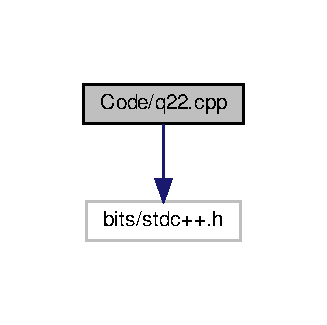
\includegraphics[width=157pt]{q22_8cpp__incl}
\end{center}
\end{figure}
\subsection*{Classes}
\begin{DoxyCompactItemize}
\item 
struct \hyperlink{struct_graph}{Graph}
\item 
struct \hyperlink{struct_disjoint_sets}{Disjoint\+Sets}
\end{DoxyCompactItemize}
\subsection*{Typedefs}
\begin{DoxyCompactItemize}
\item 
typedef pair$<$ int, int $>$ \hyperlink{q22_8cpp_a18fc5862b3095bd9855a9e15c67b392d}{i\+Pair}
\end{DoxyCompactItemize}
\subsection*{Functions}
\begin{DoxyCompactItemize}
\item 
int \hyperlink{q22_8cpp_ae66f6b31b5ad750f1fe042a706a4e3d4}{main} ()
\end{DoxyCompactItemize}
\subsection*{Variables}
\begin{DoxyCompactItemize}
\item 
ofstream \hyperlink{q22_8cpp_a1c0eed5f509d7328e7cbed76a6d11d98}{outdata}
\end{DoxyCompactItemize}


\subsection{Typedef Documentation}
\mbox{\Hypertarget{q22_8cpp_a18fc5862b3095bd9855a9e15c67b392d}\label{q22_8cpp_a18fc5862b3095bd9855a9e15c67b392d}} 
\index{q22.\+cpp@{q22.\+cpp}!i\+Pair@{i\+Pair}}
\index{i\+Pair@{i\+Pair}!q22.\+cpp@{q22.\+cpp}}
\subsubsection{\texorpdfstring{i\+Pair}{iPair}}
{\footnotesize\ttfamily typedef pair$<$int, int$>$ \hyperlink{q22_8cpp_a18fc5862b3095bd9855a9e15c67b392d}{i\+Pair}}



Definition at line 11 of file q22.\+cpp.



\subsection{Function Documentation}
\mbox{\Hypertarget{q22_8cpp_ae66f6b31b5ad750f1fe042a706a4e3d4}\label{q22_8cpp_ae66f6b31b5ad750f1fe042a706a4e3d4}} 
\index{q22.\+cpp@{q22.\+cpp}!main@{main}}
\index{main@{main}!q22.\+cpp@{q22.\+cpp}}
\subsubsection{\texorpdfstring{main()}{main()}}
{\footnotesize\ttfamily int main (\begin{DoxyParamCaption}{ }\end{DoxyParamCaption})}



Definition at line 134 of file q22.\+cpp.



\subsection{Variable Documentation}
\mbox{\Hypertarget{q22_8cpp_a1c0eed5f509d7328e7cbed76a6d11d98}\label{q22_8cpp_a1c0eed5f509d7328e7cbed76a6d11d98}} 
\index{q22.\+cpp@{q22.\+cpp}!outdata@{outdata}}
\index{outdata@{outdata}!q22.\+cpp@{q22.\+cpp}}
\subsubsection{\texorpdfstring{outdata}{outdata}}
{\footnotesize\ttfamily ofstream outdata}



Definition at line 8 of file q22.\+cpp.


%--- End generated contents ---

% Index
\backmatter
\newpage
\phantomsection
\clearemptydoublepage
\addcontentsline{toc}{chapter}{Index}
\printindex

\end{document}
